\section{Materials and Methods}\label{sec:methods}

\begin{figure*}[t]
\centering
\begin{tikzpicture}[
  node distance=4mm and 5mm, font=\footnotesize,
  box/.style={draw, rounded corners=2pt, align=center, minimum height=8mm, inner sep=3pt, fill=white},
  data/.style={box, fill=blue!6}, model/.style={box, fill=orange!10}, app/.style={box, fill=green!8},
  arr/.style={-{Stealth[length=2mm]}, thick}]
\node[data] (ds) {TrialGPT criterion\\annotations (1{,}015)};
\node[data, right=of ds] (clean) {drop GPT-4 cols\\parse numbered note};
\node[data, right=of clean] (split) {patient split 37/8/8\\seed 42 + manifest};
\node[data, right=of split] (fmt) {prompt + JSON target\\(0 truncation)};
\node[model, right=of fmt] (lora) {LoRA SFT (bf16)\\train split only};
\node[model, below=8mm of lora] (qwen) {Qwen2.5-1.5B\\+ LoRA adapter};
\node[model, left=of qwen] (kv) {KV-cached\\greedy decoder};
\node[model, left=of kv] (spec) {speculative decoder\\draft Qwen2.5-0.5B};
\node[model, left=of spec] (att) {tiled online-softmax\\attention (validated)};
\node[data, left=of att] (eval) {evaluation\\val (dev) / test (once)};
\node[app, below=8mm of kv] (api) {FastAPI service: screening facade, GPU job queue, SQLite (ORM)};
\node[app, left=of api] (ui) {Browser UI: Screen $\cdot$ Report $\cdot$ Inference Lab};
\node[app, right=of api] (out) {criterion label + sentence IDs\\+ grounded explanation\\+ rule-based outcome};
\draw[arr] (ds)--(clean); \draw[arr] (clean)--(split); \draw[arr] (split)--(fmt); \draw[arr] (fmt)--(lora);
\draw[arr] (lora)--(qwen); \draw[arr] (qwen)--(kv); \draw[arr] (kv)--(spec); \draw[arr] (spec.west)--(att.east);
\draw[arr] (kv) |- (eval.south); \draw[arr] (kv)--(api); \draw[arr] (ui)--(api); \draw[arr] (api)--(out);
\end{tikzpicture}
\caption{\sys\ architecture. The offline pipeline (top) prepares leakage-safe data and adapts the model;
the inference core (middle) contains the three hand-written mechanisms; the application (bottom) exposes
screening and live benchmarking in the browser.}
\label{fig:arch}
\end{figure*}

\subsection{Dataset and Leakage Control}\label{sec:data}
We use only \texttt{ncbi/TrialGPT-Criterion-Annotations} (revision \texttt{1cfcafd}). It contains 1{,}015
criterion-level annotations for 53 patients and 103 trials. Notes are already split into numbered sentences
(\texttt{"0. \ldots\textbackslash n1. \ldots"}), so sentence IDs are taken verbatim and evidence is a set of
those IDs. The columns \texttt{gpt4\_explanation}, \texttt{gpt4\_sentences}, \texttt{gpt4\_eligibility},
\texttt{explanation\_correctness} and TrialGPT's own \texttt{training} flag are dropped before any formatting.
A test overwrites all of these columns with a sentinel string and asserts that every one of the 1{,}015
prompts and targets is byte-identical and sentinel-free, proving that model-generated outputs cannot reach the
model. One annotation (ID 883) has an empty criterion text; it is kept, with an explicit marker, so that
counts match the source. Labels are type-specific: inclusion criteria use \{included, not included, not
enough information, not applicable\}; exclusion criteria use \{excluded, not excluded, not enough
information, not applicable\}. The label distribution is highly skewed (e.g.\ only 10 \emph{excluded}).

\subsection{Patient-Grouped Split}\label{sec:split}
Unique patient IDs are sorted lexicographically into a NumPy array, shuffled in place with
\texttt{numpy.random.default\_rng(42)}, and the first 37 / next 8 / last 8 patients form train / validation /
test. Every annotation follows its patient. Table~\ref{tab:split} gives the resulting counts; the manifest
(\texttt{data/splits/split\_manifest.json}) lists patient IDs and a SHA-256 hash of each split's annotation
IDs. Automated tests check sizes, disjointness, full coverage, determinism and that every gold evidence ID
exists in its note. Notably, the test split contains \emph{no} \emph{excluded} example, which affects how
macro-F1 must be read (Section~\ref{sec:metrics}).
\begin{table*}[t]
\centering
\footnotesize
\caption{Patient-grouped split (seed 42) and expert label counts.}
\label{tab:split}
\begin{tabular}{lrrrrrrrrrr}
\toprule
Split & Pat. & Ann. & Inc. & Exc. & incl & not incl & excl & not excl & NEI & N/A \\
\midrule
train & 37 & 603 & 215 & 388 & 88 & 13 & 8 & 292 & 174 & 28 \\
val & 8 & 206 & 66 & 140 & 35 & 3 & 2 & 101 & 53 & 12 \\
test & 8 & 206 & 75 & 131 & 27 & 7 & 0 & 91 & 66 & 15 \\
\bottomrule
\end{tabular}
\end{table*}


\subsection{Model Selection}\label{sec:model}
Table~\ref{tab:candidates} compares five open-weight decoders. Facts are read from each model's
\texttt{config.json}; parameter counts are exact (models instantiated on the \texttt{meta} device, tied
embeddings counted once). We selected \textbf{Qwen2.5-1.5B-Instruct}: Apache-2.0 and ungated; RoPE + GQA with
only 2 KV heads, giving the smallest KV cache of the candidates (28\,KiB/token in 16-bit); a 32\,K context
far above our longest example (623 tokens); 1.54\,B parameters (2.9\,GiB in bf16) that leave room on a 6\,GB
GPU for activations, the KV cache \emph{and} a draft model; and, decisively for Task~5, an official
\textbf{Qwen2.5-0.5B-Instruct} sibling with an identical tokenizer (151{,}665 entries,
identical chat template, identical 151{,}936-wide output layer). Llama-3.2-1B has no smaller same-tokenizer
sibling and a gated community licence; Gemma-2-2B (2.6\,B) and Qwen3-1.7B (1.72\,B, 8 KV
heads $\Rightarrow$ 4$\times$ larger cache) fit less comfortably next to a draft model.
\begin{table*}[t]
\centering
\footnotesize
\caption{Candidate decoders (from config.json; exact parameter counts; 16-bit memory). KV = KiB of cache per token. All use RoPE, RMSNorm/LayerNorm variants and GQA.}
\label{tab:candidates}
\begin{tabular}{lrrcrrrrrl}
\toprule
Model & Params (B) & L & Hq/Hkv & d & Vocab & Ctx & GiB & KV & Licence \\
\midrule
Qwen2.5-1.5B-Instruct & 1.54 & 28 & 12/2 & 128 & 151k & 32k & 2.9 & 28 & Apache-2.0 \\
Qwen2.5-0.5B-Instruct & 0.49 & 24 & 14/2 & 64 & 151k & 32k & 0.9 & 12 & Apache-2.0 \\
Qwen3-1.7B & 1.72 & 28 & 16/8 & 128 & 151k & 40k & 3.2 & 112 & Apache-2.0 \\
Llama-3.2-1B-Instruct & 1.24 & 16 & 32/8 & 64 & 128k & 128k & 2.3 & 32 & Llama 3.2 CL \\
gemma-2-2b-it & 2.61 & 26 & 8/4 & 256 & 256k & 8k & 4.9 & 104 & Gemma ToU \\
\bottomrule
\end{tabular}
\end{table*}


\subsection{Input/Output Format and Tokenisation}\label{sec:format}
One prompt template (Qwen chat format) is shared by fine-tuning, evaluation and the application. The system
message instructs the model to judge one criterion from the numbered note only, to answer \emph{not enough
information} when facts are missing (``missing evidence is never proof''), and to reply with JSON. The user
message contains the numbered note, the criterion type, the criterion text and the four allowed labels for
that type. The target is a compact JSON object, e.g.\
\texttt{\{"label": "included", "evidence": [0, 3]\}}. With Qwen's byte-level BPE tokenizer the longest
training example is 623 tokens (median 311; Fig.~\ref{fig:tokens}); we set \texttt{max\_seq\_len}=1024, so
\textbf{no example is truncated and no evidence sentence is lost}---verified by an audit that would list any
truncated annotation and any gold sentence beyond the cut. A robust parser extracts the first JSON object,
normalises label synonyms, rejects labels not allowed for the criterion type (counted as \emph{invalid}, never
silently mapped), and drops cited IDs that do not exist in the note (reported as unsupported citations).

\begin{figure}[t]
\centering
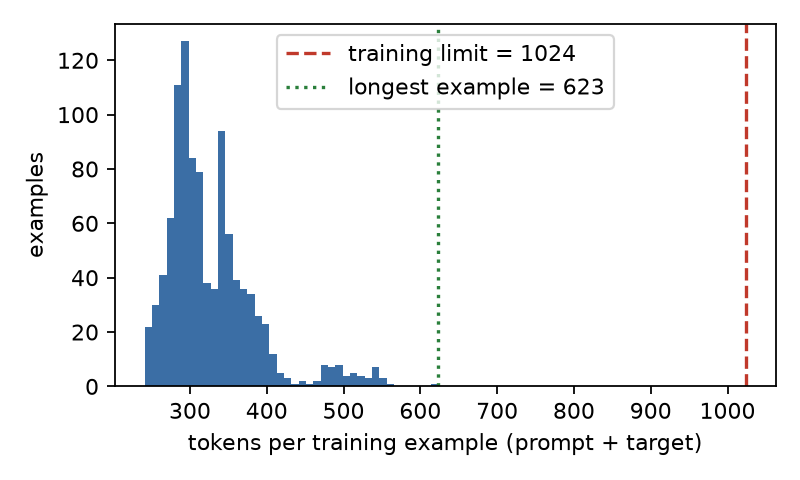
\includegraphics[width=0.92\linewidth]{token_hist.png}
\caption{Tokens per training example (prompt + target) across all 1{,}015 annotations. The dashed line is
the training limit; every example fits, so truncation never removes evidence.}
\label{fig:tokens}
\end{figure}

\subsection{Fine-Tuning}\label{sec:ft}
\textbf{Objective.} Supervised fine-tuning with the causal LM cross-entropy computed only on assistant
(target) tokens; all prompt tokens are masked with $-100$, so the model learns to emit the label and
evidence, not to reproduce notes. The \texttt{<|im\_end|>} token is part of the target, teaching the model
to stop.

\textbf{Precision strategy chosen by measurement.} Our GTX~1660~SUPER (6\,GB, Turing \texttt{sm\_75}, no
tensor cores) behaves unlike the GPUs in the literature. A micro-benchmark gave 3.9\,TFLOP/s for fp32 GEMM,
2.1 for bf16 but only 0.43 for fp16 (cuBLAS fp16 with fp32 accumulation is slow on TU116). We therefore ran
every candidate training configuration for four optimizer steps on the \emph{longest} training example in
a fresh process (Table~\ref{tab:membench}). The Windows driver's ``CUDA sysmem fallback'' initially let fp32
silently spill into system RAM (a 100$\times$ slowdown instead of an error); capping the allocator at the
physical VRAM made out-of-memory explicit. Full fp32 does not fit (6.2\,GiB of weights); accelerate's CPU
offload is incompatible with PEFT gradients; fp16 autocast works but is 3.6$\times$ slower; QLoRA saves
0.9\,GB but quantises the frozen weights. \textbf{bf16 storage of the frozen base + fp32 LoRA weights +
bf16 autocast + gradient checkpointing} is the fastest configuration that keeps the original weights; any
micro-batch above one exceeds memory because the 151{,}936-way output logits dominate activations, so we use
micro-batch 1 with 16 accumulation steps.
\begin{table}[t]
\centering
\footnotesize
\caption{Measured training configurations on NVIDIA GeForce GTX 1660 SUPER (6.0 GB): LoRA r=16, longest training example (623 tokens), 4 optimizer steps, first step excluded from timing.}
\label{tab:membench}
\begin{tabular}{lcrrrrl}
\toprule
Strategy & Ckpt & MB & Weights GiB & Peak GiB & s/step & Status \\
\midrule
fp32 & yes & 1 & -- & -- & -- & OOM \\
fp32-offload & yes & 1 & -- & -- & -- & incompatible \\
fp16-mixed & yes & 1 & 2.94 & 4.22 & 13.80 & ok \\
bf16-mixed & no & 1 & -- & -- & -- & OOM \\
bf16-mixed & yes & 1 & 2.94 & 4.22 & 3.87 & ok \\
bf16-mixed & yes & 4 & -- & -- & -- & OOM \\
bf16-mixed & yes & 8 & -- & -- & -- & OOM \\
qlora-nf4 & yes & 1 & 1.58 & 3.33 & 3.71 & ok \\
qlora-nf4 & yes & 4 & -- & -- & -- & OOM \\
\bottomrule
\end{tabular}
\end{table}


\textbf{Hyper-parameters} (Table~\ref{tab:hparams}): LoRA rank 16, $\alpha$=32, dropout 0.05 on all seven
attention and MLP projections (18.5\,M trainable parameters, 1.2\% of the model), AdamW~\cite{loshchilov2019adamw}
with learning rate $2\times10^{-4}$, cosine schedule with 5\% warm-up, gradient clipping at 1.0, 3 epochs,
seed 42. After each epoch the adapter is saved and the \emph{validation} split is decoded with the exact
evaluation decoder; the epoch with the best validation macro-F1 (ties: evidence micro-F1) is selected.
The test split is never used for selection.
\begin{table}[t]
\centering
\footnotesize
\caption{Fine-tuning configuration.}
\label{tab:hparams}
\begin{tabular}{ll}
\toprule
Setting & Value \\
\midrule
Base model & Qwen/Qwen2.5-1.5B-Instruct \\
Precision & bf16 base, fp32 LoRA, bf16 autocast \\
LoRA r / $\alpha$ / dropout & 16 / 32 / 0.05 \\
Target modules & q,k,v,o,gate,up,down \\
Optimizer & AdamW, wd 0.0 \\
LR / schedule & 0.0002 / cosine, 5\% warm-up \\
Batch & 1 $\times$ 16 accumulation \\
Epochs / clip / seed & 3 / 1.0 / 42 \\
Max length & 1024 (no truncation) \\
Grad. checkpointing & True \\
Selection & best val macro-F1 over epochs \\
\bottomrule
\end{tabular}
\end{table}


\subsection{Grounded Explanations}\label{sec:explain}
The dataset's only free-text explanations are GPT-4 outputs, which we refuse to use as targets (leakage,
and 124 of them are marked partially correct or incorrect). The fine-tuned model therefore emits only label
and evidence, and the explanation is produced afterwards in one of two ways. (i) \emph{Grounded LLM}: the
same network with the LoRA adapter \emph{disabled} (i.e.\ the instruction-tuned base) receives only the
criterion, the decided label and the text of the cited sentences, and writes one or two sentences. A
deterministic grounding check rejects any rationale that mentions a number absent from the cited evidence or
the criterion, or that contradicts the label. (ii) \emph{Template}: a deterministic sentence quoting the cited
evidence verbatim. Rejected LLM rationales fall back to the template, so every explanation shown is grounded
in the cited sentences.

\subsection{KV-Cached Autoregressive Decoding}\label{sec:kv}
We implement greedy decoding directly on model forward passes (Alg.~\ref{alg:kv}). In prefill the full prompt
of length $T$ is processed with \texttt{position\_ids} $=0..T-1$; each layer stores keys (already rotated by
RoPE) and values in a \texttt{DynamicCache} of shape $[B, H_{kv}, T, d]$. Each decode step feeds only the
newest token with absolute position $T+t$ (\texttt{position\_ids} and \texttt{cache\_position}) and an
attention mask extended by one; the cache grows by one entry per layer. Because RoPE is applied before
caching, cached keys retain their absolute positions; a wrong position for the new query silently changes
the output, which our equality tests would detect. A causal mask is needed in prefill but not for a single
query at the last position. The reference path re-runs the whole sequence without cache at every step.
Assertions check the cache length after prefill and after decoding, and a trace records the layer-0 key
shape at every step (Section~\ref{sec:res-kv}). With GQA, the cache stores $H_{kv}=2$ heads instead of
$H_q=12$: $2\cdot L\cdot H_{kv}\cdot d\cdot 2$\,B $=28$\,KiB per token for $L$=28, $d$=128.

\begin{algorithm}[t]
\caption{KV-cached greedy decoding (batch 1)}\label{alg:kv}
\begin{algorithmic}[1]
\State $C\gets$ empty cache; $\ell \gets f(x_{0:T};\ \mathrm{pos}=0..T{-}1, C)$ \Comment{prefill, appends $T$ K/V}
\State $y_1\gets\arg\max \ell_{T-1}$
\For{$t=1$ \textbf{to} $N-1$ \textbf{while} $y_t\notin\mathrm{EOS}$}
  \State $\ell\gets f(y_t;\ \mathrm{pos}=T{+}t{-}1, C)$ \Comment{one token; cache grows by 1}
  \State $y_{t+1}\gets\arg\max \ell$
\EndFor
\State \textbf{assert} $|C| = T + |y| - 1$
\end{algorithmic}
\end{algorithm}

\subsection{Tiled Attention with Online Softmax}\label{sec:attn}
The reference computes $S=QK^\top/\sqrt{d}$ in fp32, masks with $-\infty$ (causal convention: query $i$ at
absolute position $S_k-S_q+i$ may see keys $j\le S_k-S_q+i$, which also covers single-token decode), subtracts the
row maximum before exponentiation, normalises, and multiplies by $V$; fully masked rows return zeros. The
tiled kernel (Alg.~\ref{alg:tiled}) never forms $S$: for each block of $B_q$ queries it streams blocks of $B_k$
keys, keeping a running maximum $m$, normaliser $\ell$ and un-normalised output $A$. When a new block raises
the maximum, previous statistics are rescaled by $\alpha=e^{m-m'}$~\cite{milakov2018online,dao2022flashattention}.
Key blocks entirely above the diagonal are skipped; only diagonal blocks are masked. GQA is handled by
repeating KV heads. All accumulation is in fp32.

\begin{algorithm}[t]
\caption{Tiled attention with online softmax (one query block)}\label{alg:tiled}
\begin{algorithmic}[1]
\State $m\gets-\infty,\ \ell\gets0,\ A\gets0$ \Comment{per query row}
\For{each key block $j$ visible under the causal mask}
  \State $S_j\gets Q_iK_j^\top/\sqrt d$; mask inside the diagonal block
  \State $m'\gets\max(m,\mathrm{rowmax}(S_j))$;\ $P\gets e^{S_j-m'}$;\ $\alpha\gets e^{m-m'}$
  \State $\ell\gets\alpha\ell+\mathrm{rowsum}(P)$;\ $A\gets\alpha A+PV_j$;\ $m\gets m'$
\EndFor
\State $O_i\gets A/\ell$;\quad $\mathrm{LSE}_i\gets m+\log\ell$
\end{algorithmic}
\end{algorithm}

\subsection{Greedy Speculative Decoding}\label{sec:spec}
Draft $D$ (Qwen2.5-0.5B-Instruct, 0.49\,B) and target $M$ (fine-tuned 1.5\,B) keep separate KV caches. With
$s$ the current sequence of length $L$, the invariant is that $M$'s cache holds $s_{0:L-1}$ and $D$'s holds
$s_{0:L-1}$ or $s_{0:L-2}$; the last token is pending. Each round (Alg.~\ref{alg:spec}): $D$ ingests its pending
token(s) and greedily proposes $\gamma$ tokens; $M$ runs \emph{one} forward over $[s_{L-1}, d_1..d_\gamma]$ at
positions $L{-}1..L{-}1{+}\gamma$, yielding its own greedy choices $g_1..g_{\gamma+1}$; the longest prefix with
$d_i=g_i$ is accepted and $g_{n+1}$ is appended (a correction if $n<\gamma$, a free bonus token if $n=\gamma$).
Both caches are then cropped (\texttt{DynamicCache.crop}) so that no key/value of a rejected token survives.
EOS or the token budget inside an accepted block truncates exactly. Every emitted token is the target's own
greedy choice for the same prefix, so the output must equal plain greedy decoding; cache-length assertions run
after every round.

\begin{algorithm}[t]
\caption{Greedy speculative decoding: one round}\label{alg:spec}
\begin{algorithmic}[1]
\State $D$: ingest pending token(s); propose $d_{1..\gamma}$ greedily
\State $M$: one forward on $[s_{L-1}, d_{1..\gamma}]$ $\Rightarrow$ $g_{1..\gamma+1}$
\State $n\gets\max\{k: d_{1..k}=g_{1..k}\}$; \ $s\gets s\,\Vert\, d_{1..n}\,\Vert\, g_{n+1}$
\State $M$.crop$(|s|-1)$;\ $D$.crop$(\min(|D|,|s|-1))$ \Comment{drop rejected K/V}
\State stats: proposed $+{=}\gamma$, accepted $+{=}n$
\end{algorithmic}
\end{algorithm}

\subsection{Application Workflow}\label{sec:app}
The FastAPI service follows a router\,$\rightarrow$\,service\,$\rightarrow$\,repository layering with Pydantic
request schemas (constraints double as input validation: note 20--12{,}000 characters, 1--40 criteria, typed
labels, NCT-ID pattern, $\gamma\in[1,8]$). A singleton model registry loads the target (with the adapter kept
\emph{unmerged} so explanations can disable it) and the draft once, in the background; a single-worker
executor serialises GPU jobs. A screening is created as a job whose criteria are decoded one by one and
persisted (SQLite through SQLAlchemy), while the browser polls progress. Free-text notes are segmented into
numbered sentences; criteria can be pasted (split on Inclusion/Exclusion headings), typed, or fetched by NCT ID
from the public ClinicalTrials.gov API. The overall preliminary outcome is an explicit rule, never a predicted
label: any inclusion \emph{not included} or exclusion \emph{excluded} $\Rightarrow$ \emph{Likely ineligible};
otherwise any \emph{not enough information} (or unparseable output) $\Rightarrow$ \emph{Needs more
information}; otherwise \emph{Likely eligible}; \emph{not applicable} is neutral. Reports are exported as
printable HTML, Markdown or JSON with provenance (model, adapter SHA-256, precision, decoding settings, commit,
timestamp) and the disclaimer. The Inference Lab runs no-cache, KV-cached and speculative decoding live on a
validation prompt or a custom prompt, and the reference/tiled/PyTorch attention kernels against a float64
ground truth.
